%
% DS 5110 (Blue Team) Project Proposal
%
\documentclass[12pt]{article}

%
% Packages
%
\usepackage{amsmath}
\usepackage{enumerate}
\usepackage[utf8]{inputenc}

\RequirePackage{graphics}

\usepackage{graphicx}
\graphicspath{ {imgs/} }

%
% Document Settings
%
\setlength{\parskip}{1pc}
\setlength{\parindent}{0pt}
\setlength{\topmargin}{-3pc}
\setlength{\textheight}{9.5in}
\setlength{\oddsidemargin}{0pc}
\setlength{\evensidemargin}{0pc}
\setlength{\textwidth}{6.5in}

\title{DS 5110: Project - Fall 2017}
\author{Tyler Brown, Sicheng Hao, Nischal Mahaveer Chand, Sumedh Sankhe}
\date{ }


% START DOCUMENT
\begin{document}

\maketitle

\section{Summary}

I am new to Boston and I'm looking for properties and I have no idea
what each neighborhood's are about. When I checked Zillow and Trulia,
I found which homes were for sale. I was able to filter by location,
price range, details about the home such as beds and bathrooms, types
of homes like condos, apartments, and houses. I was also able to find
information on mortgages, real estate agents, and home designs such
as traditional and modern.

When I visited another major real estate website, Trulia, there were
many similarities to Zillow. One major difference is that Trulia
provides a ``Local Scoop'' which gives me details about market trends,
schools, and crime in the greater Boston area. When I select ``Local
Scoop'', I found a dashboard with a map showing were crime is most
prevelant or the exact location of schools. I also noticed that I could
look at individual records from the data below the dashboard map. When
I checked out ``Boston Real Estate Market Overview'', I found information
about where to find the most expensive homes. There were line graphs
showing how prices flutuated over time. I was also able to get to know
my potential neighbors in Boston because they provided demographic
information such as the percentage of single residents, home owners,
median age, and median household income. They also provided a heatmap
of commuting times and types of commute. Additionally, they recommended
nearby cities where I might like to live.

This was a lot of information to consider. However, I found myself unable
to ask more detailed questions such as when a home was remodelled, or
when my neighbors were making changes to their homes. Are there
neighborhoods owned by individuals or companies? Have certain companies
been taking over specific neighborhoods? \textbf{How have the
  neighborhoods been changing over time?} The answer to this question
is actionable because changes in a neighborhood provide insight into
the types of neighbors I'll have and how my home value could change
based on the activities going on around me. \textbf{I want to better understand my potentially new community}.




The City of Boston provides an open data platform, Analyze Boston, 
containing information related to our lives in the city. Property 
assessment data from 2014-2017 is one of the resources available on their
 open data platform. Included in the property assessment data is 
``property, or parcel, ownership together with information about value, 
which ensures fair assessment of Boston taxable and non-taxable property 
of all types and classifications'' \cite{Property49:online}. Our team 
has aggregated each available year to create a time series dataset of 
Property Assessments in Boston. This aggregated dataset allows us to 
provide unique insights into property valuations and ownership strategies.

The problem our group is focusing on is how we can help people who are 
looking for buying houses or condos by present an overlook of Boston 
housing market reflected by their assessment values.

\section{Proposed Plan of Research}

 The datasets we are having right now are separate yearly. The first step 
we are going to do is merge them into one single file. Then we are going 
to do some necessary cleaning for the data set. 

In the second step, we are going to filter out the data that could 
represent the problem we are trying to solve. Maybe add some data from 
other sources( like Google Maps or Zillow)

To help people understand the data better. In the last step we will make 
an interactive Shiny application to visualize our finding. 


\section{Preliminary Results}

Our preliminary results include a data audit and descriptive findings.
The data audit found trouble spots in our data such as missing values or
incomplete values for coordinates as well as a small number of duplicate
values for the given primary keys. The descriptive findings generated
possible directions for our research question such as changes in 
property valuations, dominant ownership strategies for owners 
controlling a higher percentage of Boston property, and changes in
property valuations for various land usage types.

\subsection{Data Audit Findings}

The major data audit findings are (1) the given primary keys, $PID$, are 
not unique for 0.3\% because they are mapped to multiple geographic 
coordinate pairs, (2) about 22\% of geographic coordinates are either 
missing or unusable, (3) about 10\% of property parcels, identified with
$PID$ do not pay taxes. Of that 10\%, we can explain about 49\% of this 
variation due to tax-exempt land use status. The remaining 51\% is 
associated with the "Condominium main" land usage type. It's unclear why 
there are zero taxes associated with this land usage type without 
contacting the city of Boston. This anomaly effects about 5\% of the 
total data.

\subsection{Descriptive Findings}
Preliminary relationships found within the data are (1) residential 
condominium units appear to have the lowest proportion of value but 
previously we saw they had the second-highest proportion of gross tax,
(2) residential family and residential land appears to have gained the 
most value from 2014-2017, (3) the most significant gains in property
assessment from 2014-2017 have been made land used for commerical and
commerical condominium properties, (4) those who are further away from 
the financial district appear to be generally paying a lower proportion 
of taxes, and (5) larger real estate developers appear to choose one
of two distinct strategies that involve either paying higher taxes with
less property or lower taxes with more property. The figure below shows
how location might effect changes in property assessments from 2014-2017.

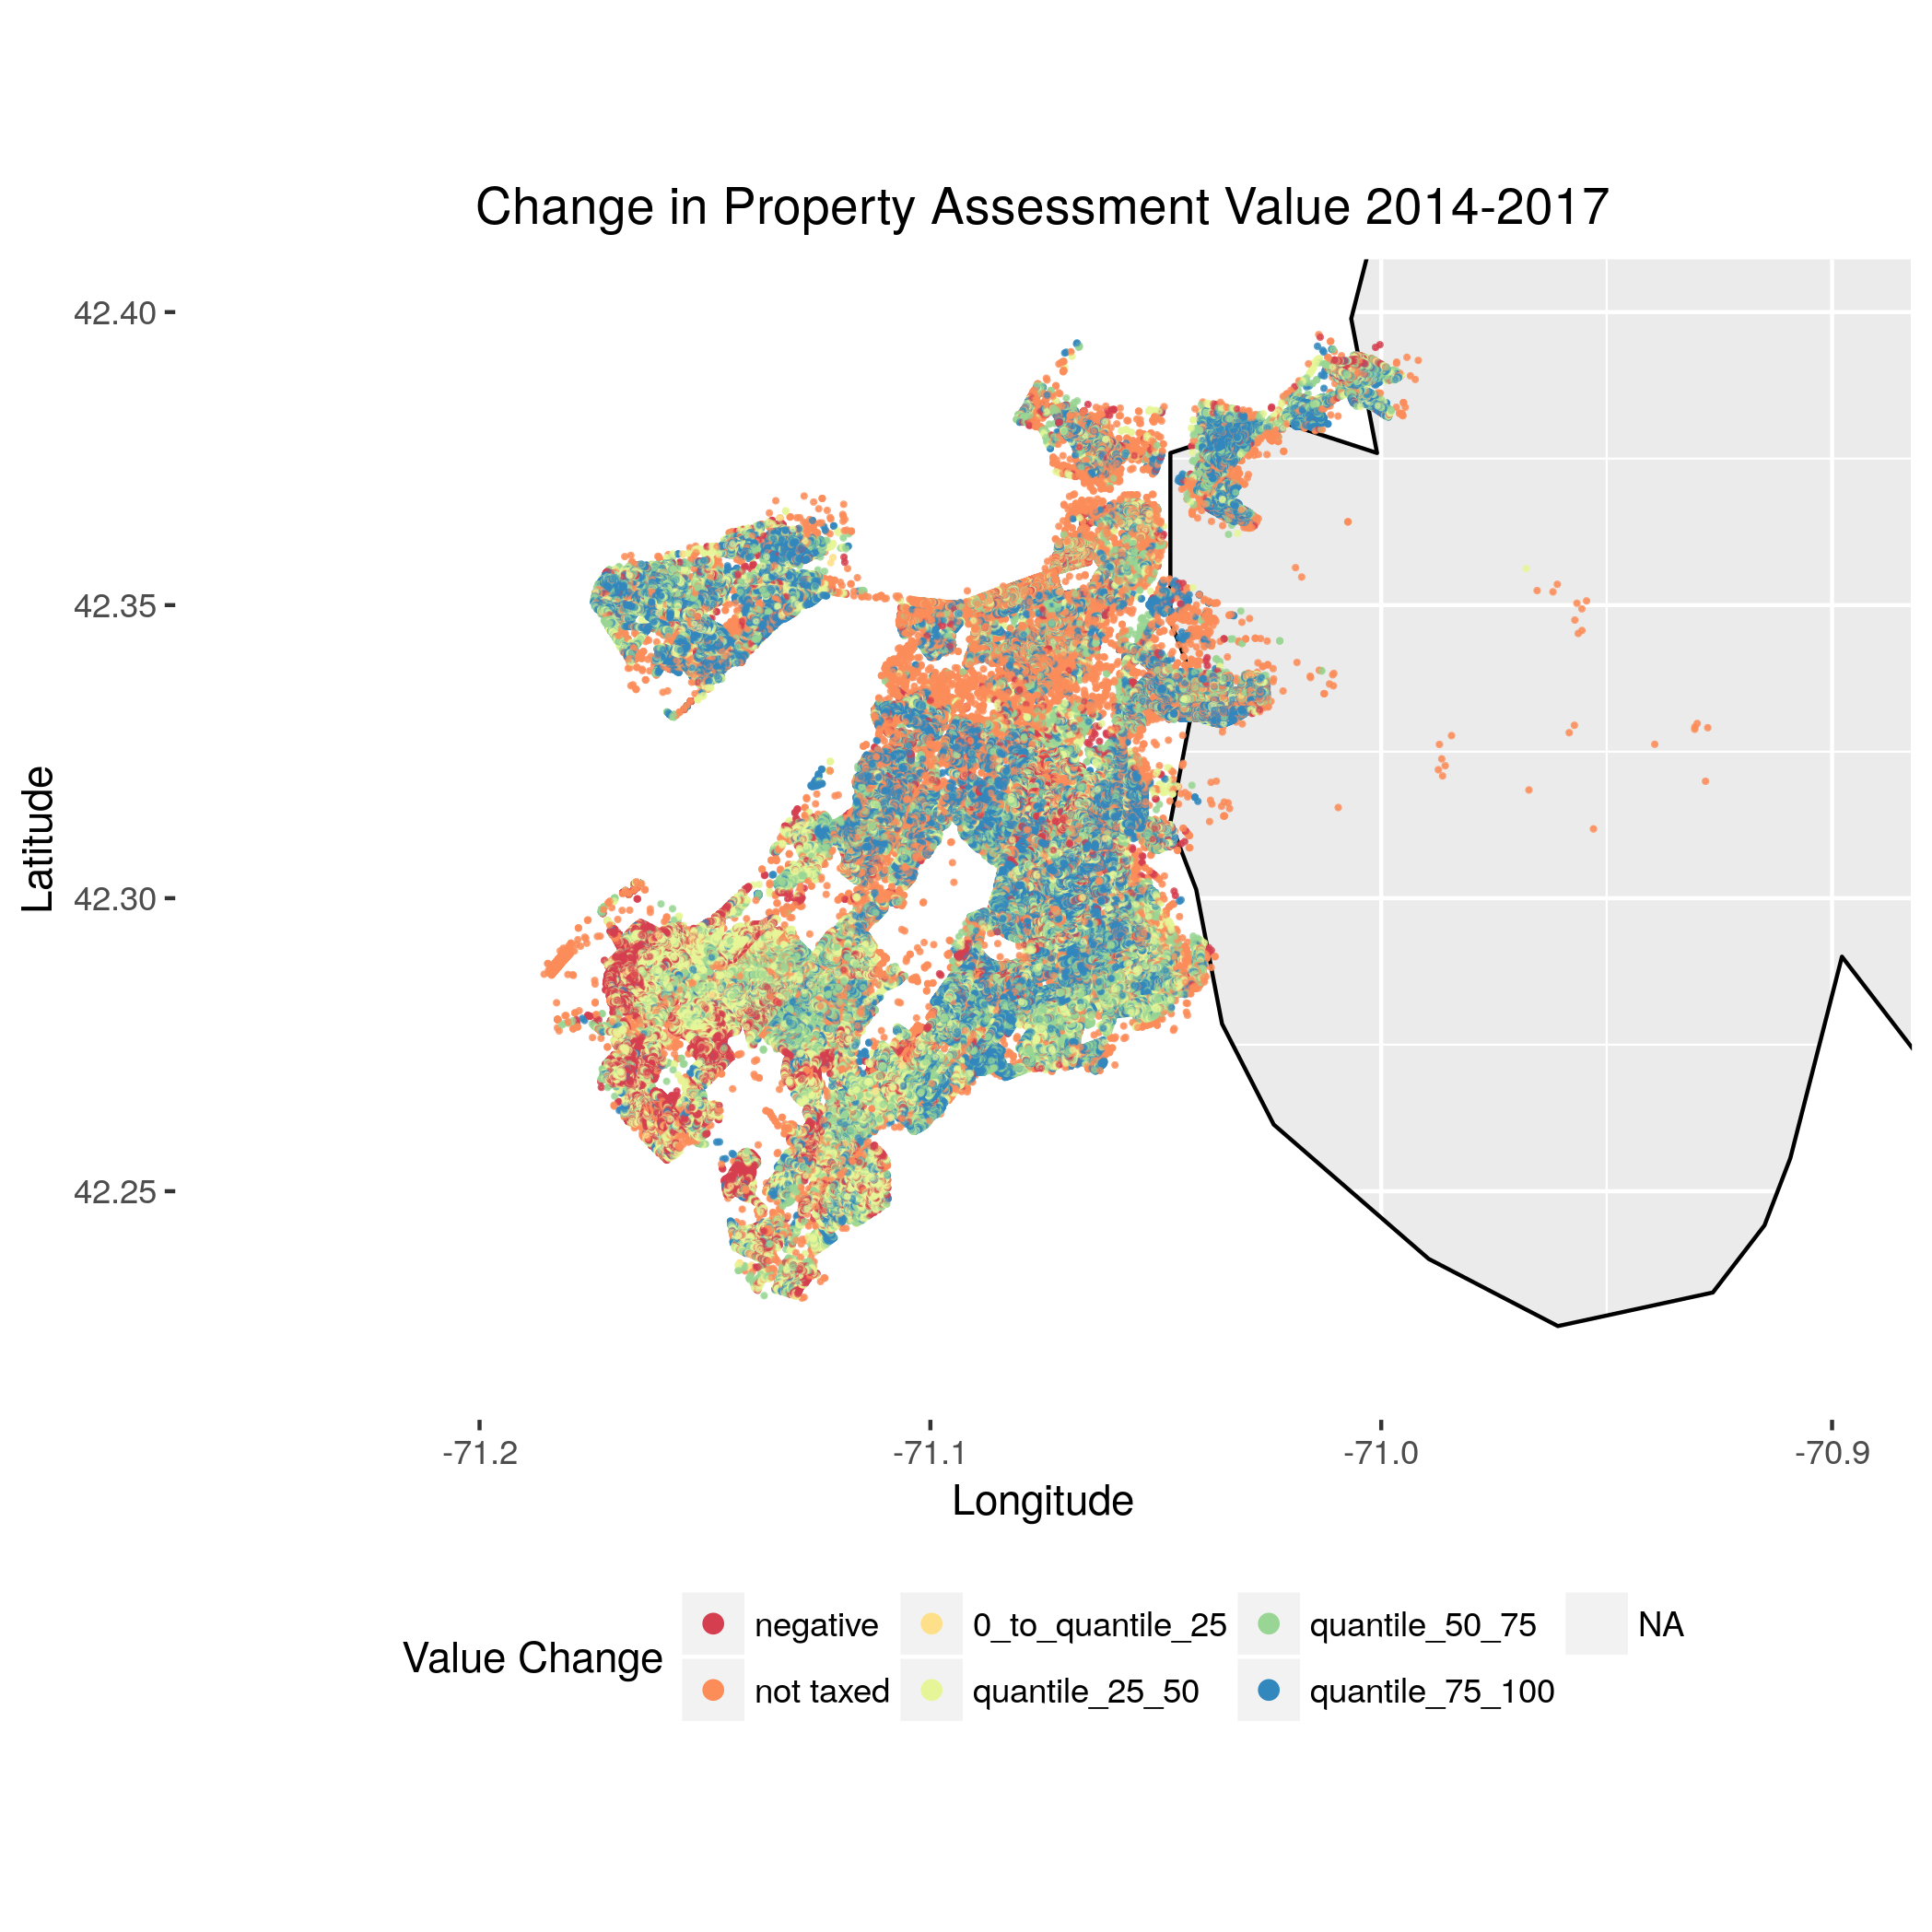
\includegraphics[scale=0.75]{property_delta2014-2017}


\bibliography{references} 
\bibliographystyle{ieeetr}

\end{document}
